\documentclass[11pt]{article}

\usepackage{amsmath}
\usepackage{amssymb}
\usepackage{fancyhdr}
\usepackage{comment}
\usepackage{color}
\usepackage{graphicx}
\usepackage{tikz}
\usepackage{booktabs}
\usepackage{listings}
\usepackage[colorlinks=true,linkcolor=blue,urlcolor=blue]{hyperref}
\usetikzlibrary{arrows, automata}
%\usetikzlibrary{arrows.meta}

\newcounter{marks}
\def\maxmarks#1{\extramark{#1}\addtocounter{marks}{#1}}
\def\extramark#1{\hfill
  [\emph{#1 points}]
%  \quad\mbox{\LARGE\begin{tabular}{|c|c|}
%  \hline\rule{1cm}{0cm} & #1 \\ \hline \end{tabular}}
}
\def\dumptotal{%
\begin{flushright}
\begin{tabular}{|l|} \hline
\LARGE{\textbf{\rule{0pt}{16pt}Total:~\themarks}} \\ \hline
\end{tabular}
\end{flushright}}
\def\skiplines#1{\newline \forloop{#1}{{\rule{0pt}{20pt}} \\}}

\specialcomment{answer}{\color{blue}}{\color{black}}
\def\withanswers{\def\skiplines##1{\relax}\def\skippage{\relax}}
\def\withoutanswers{\excludecomment{answer}\def\skippage{\clearpage}}

\newif\ifprint
\printfalse

\oddsidemargin0cm
\topmargin-2cm     %I recommend adding these three lines to increase the 
\textwidth16.5cm   %amount of usable space on the page (and save trees)
\textheight23.5cm  

\newcommand{\mycoursenum}{10-601}
\newcommand{\myhwnum}{7}
\newcommand{\myname}{Dawei Wang}
\newcommand{\myandrew}{daweiwan@andrew.cmu.edu}
\newcommand{\myfirstta}{Kuo Liu}
\newcommand{\mysecondta}{Harry Gifford}

\newcommand{\question}[2] {\vspace{.25in} \hrule\vspace{0.5em} \noindent{\bf #1: #2} \vspace{0.5em} \hrule \vspace{.10in}}
\renewcommand{\part}[1] {\vspace{.10in} {\bf (#1)}}

\setlength{\parindent}{0pt}
\setlength{\parskip}{5pt plus 1pt}
 
\pagestyle{fancyplain}
\lhead{\fancyplain{}{\textbf{HW\myhwnum}}}
\ifprint
\rhead{\fancyplain{}{Andrew ID: \rule{0.2\textwidth}{.4pt}}}
\else
\rhead{\fancyplain{}{\myname\\ \myandrew}}
\fi
\chead{\fancyplain{}{\mycoursenum}}

\withoutanswers

\begin{document}

\medskip

\thispagestyle{plain}
\begin{center}
{\Large \mycoursenum: Homework \myhwnum} \\
Due: 17 November 2014 11:59pm (Autolab) \\
TAs: \myfirstta, \mysecondta \\
\medskip
\ifprint
Name: \rule{0.5\textwidth}{.4pt} \\
Andrew ID: \rule{0.45\textwidth}{.4pt} \\
\else
Name: \myname \\
Andrew ID: \myandrew \\
\fi
\end{center}

Please answer to the point, and do not spend time/space giving irrelevant details. 
%You should not require more space than is provided for each question. If you do, please think whether you can make your argument more pithy, an exercise that can often lead to more insight into the problem. 
Please state any additional assumptions you make while answering the questions. 
For Questions 1 to 5, 6(b) and 6(c), you need to submit your answers in a single PDF file on autolab, either a scanned handwritten version or a \LaTeX pdf file. 
Please make sure you write legibly for grading.
For Question 6(a), submit your m-files on autolab. 

You can work in groups. However, no written notes can be shared, or taken during group discussions. You may ask clarifying questions on Piazza. However, under no circumstances should you reveal any part of the answer publicly on Piazza or any other public website. The intention of this policy is to facilitate learning, not circumvent it. Any incidents of plagiarism will be handled in accordance with \href{http://www.cmu.edu/policies/documents/Academic%20Integrity.htm}{CMU's Policy on Academic Integrity}.


%%%%%%%%%%%%%%%%%%%%%%%%%%%%%%%%%%%%%%%%%%%
\question{$\star$}{Code of Conduct Declaration}

\begin{itemize}
	\item Did you receive any help whatsoever from anyone in solving this assignment? No.
	\item Did you give any help whatsoever to anyone in solving this assignment? No.
\end{itemize}


\clearpage
%%%%%%%%%%%%%%%%%%%%%%%%%%%%%%%%%%%%%%%%%%%
\question{1}{Warmup (TA:- Either)}

Which of the following independence statements are true in the following directed graphical model? Explain your answer. $A \perp B \mid C$ can be read as ``$A$ is independent of $B$ given $C$''.

\begin{figure}[h]
\centering
\begin{tabular}{cc}
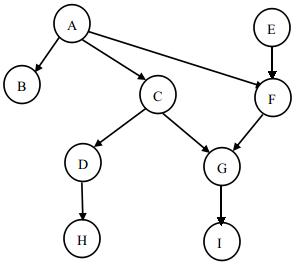
\includegraphics[width = 0.48\textwidth]{q2.jpg}& 
\end{tabular}
\caption{A simple DAG}\label{fig:GNB}
\end{figure}

\part{a} $A \perp E$ \maxmarks{3}

{\color{blue} TRUE. There doesn't exist a path between $A$ and $E$
that doesn't contain a collider. } \vspace{0 cm}

\part{b} $A \perp E \mid G$ \maxmarks{3}

{\color{blue} FALSE. $G$ is a collider, and there exists a path $A$-$C$-$G$-$F$-$E$ 
that contains it. } \vspace{0 cm}

\part{c} $C \perp F \mid \{A, G\}$ \maxmarks{3} 

{\color{blue} FALSE. $G$ is a collider, and there exists a path $C$-$G$-$F$ that contains it. }
\vspace{0 cm}

\part{d} $B \perp F \mid \{C,E\}$ \maxmarks{3}

{\color{blue} FALSE. There exists a path $B$-$A$-$F$ that doesn't contain a collider nor
$C$ and $E$. } \vspace{0 cm}

\part{e} $A \perp D \mid C$ \maxmarks{3}

{\color{blue} TRUE. C is not a collider, and there doens't exist a path
that doesn't contain $C$. } \vspace{0 cm}

\clearpage
%%%%%%%%%%%%%%%%%%%%%%%%%%%%%%%%%%%%%%%%%%%
\question{2}{Bayesian Networks (TA:- \mysecondta)}

\part{a} Prove that the any Bayesian network represents a valid probability distribution. Your proof should be general enough to apply to any graphical model, but to avoid clunky notation you may just prove it for the following graphical model. Specifically, you should show $\forall i, \forall X_i, \Pr(X_1, ..., X_n) \geq 0$ and $\sum_{X_1}\sum_{X_2}...\sum_{X_n} \Pr(X_1, ..., X_n) = 1$.
\begin{center}
    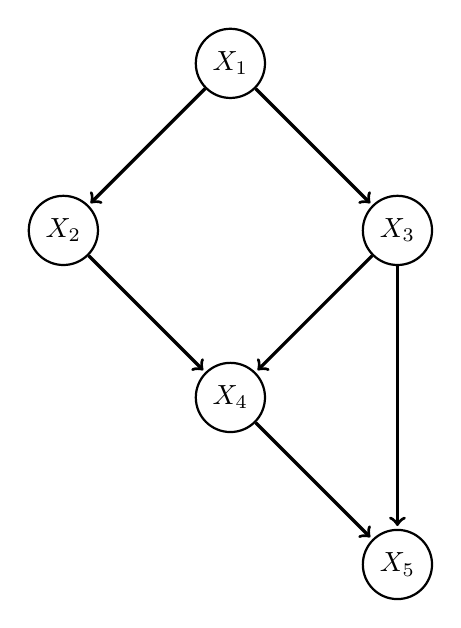
\begin{tikzpicture}[
            shorten > = 1pt, % don't touch arrow head to node
            auto,
            node distance = 3cm, % distance between nodes
            semithick % line style
        ]

        \tikzstyle{every state}=[
            draw = black,
            thick,
            fill = white,
        ]

        \node[state] (X1) {$X_1$};
        \node[state] (X2) [below left of=X1] {$X_2$};
        \node[state] (X3) [below right of=X1] {$X_3$};
        \node[state] (X4) [below right of=X2] {$X_4$};
        \node[state] (X5) [below right of=X4] {$X_5$};
        \begin{scope}[very thick]

        \path[->] (X1) edge (X2);
        \path[->] (X1) edge (X3);
        \path[->] (X2) edge (X4);
        \path[->] (X3) edge (X4);
        \path[->] (X3) edge (X5);
        \path[->] (X4) edge (X5);
\end{scope}
    \end{tikzpicture}
\end{center}

\maxmarks{10} \vspace{0 cm}

{\color{blue} 

\begin{flalign*}
	\Pr(X_1,\dots,X_n)&=\prod_{X_i}\Pr\left(X_i\big|\text{Parents}\left(X_i\right)\right)\\
	&=\Pr(X_1)\Pr(X_2|X_1)\Pr(X_3|X_1)\Pr(X_4|X_2,X_3)\Pr(X_5|X_4,X_3)\ge0
\end{flalign*}
These conditional probabilities are equal or greater than zero according to the probability axioms. 
\begin{flalign*}
	&\sum_{X_1}\sum_{X_2}\cdots\sum_{X_n}\Pr(X_1,\dots,X_n) \\ =&
	\sum_{X_1}\sum_{X_2}\cdots\sum_{X_5}
		\Pr(X_1)\Pr(X_2|X_1)\Pr(X_3|X_1)\Pr(X_4|X_2,X_3)\Pr(X_5|X_4,X_3) \\ =&
	\sum_{X_1}\Pr(X_1)\sum_{X_2}Pr(X_2|X_1)\sum_{X_3}\Pr(X_3|X_1)
		\sum_{X_4}\Pr(X_4|X_2,X_3)\sum_{X_5}\Pr(X_5|X_4,X_3) \\ =&
	\sum_{X_1}\Pr(X_1)\sum_{X_2}Pr(X_2|X_1)\sum_{X_3}\Pr(X_3|X_1)
		\sum_{X_4}\Pr(X_4|X_2,X_3)\cdot1=\cdots=1
\end{flalign*}
}

\newpage
\part{b} Now we will explore the idea of equivalence for Bayesian networks. First some definitions. We say that two graphical models $G_1$ and $G_2$ are \textit{Markov equivalent} if every independence statement in $G_1$ is also expressed in $G_2$ and likewise for $G_2$ into $G_1$. We define a \textit{V-configuration}, $\langle i, j, k \rangle$ as a subgraph with three vertices and two edges connecting $i, j$ and $j, k$. We say a V-configuration $\langle i, j, k\rangle$ is \textit{shielded} if $i$ is connected to $k$ or $k$ is connected to $i$. Two graphs have the same \textit{skeleton} if the graphs obtained from removing the directions from the edges are the same.

Finally, we say two graphs $G_1$ and $G_2$ are Markov Equivalent iff

\begin{enumerate}
\item $G_1$ and $G_2$ have the same skeleton.
\item $G_1$ and $G_2$ have the same unshielded collider (i.e. $i \rightarrow j \leftarrow k$) V-configurations.
\end{enumerate}

For each pair of graphs below (i.e. $(G_1, G_2)$, $(G_1, G_3)$, $(G_2, G_3)$) state whether they are Markov equivalent or not. Explain your answer.

    $G_1$

\begin{center}    
    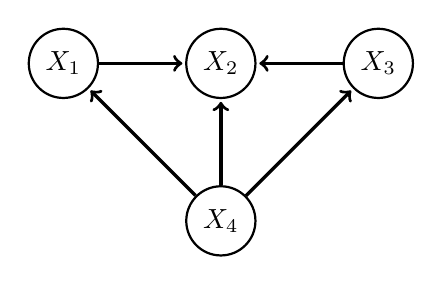
\begin{tikzpicture}[
            shorten > = 1pt, % don't touch arrow head to node
            auto,
            node distance = 2cm, % distance between nodes
            semithick % line style
        ]

        \tikzstyle{every state}=[
            draw = black,
            thick,
            fill = white,
        ]

        \node[state] (X1) {$X_1$};
        \node[state] (X2) [right of=X1] {$X_2$};
        \node[state] (X3) [right of=X2] {$X_3$};
        \node[state] (X4) [below of=X2] {$X_4$};
        \begin{scope}[very thick]

        \path[->] (X1) edge (X2);
        \path[->] (X3) edge (X2);
        \path[->] (X4) edge (X1);
        \path[->] (X4) edge (X2);
        \path[->] (X4) edge (X3);
        \end{scope}

    \end{tikzpicture}
    \end{center}
    
    $G_2$
    
\begin{center}
    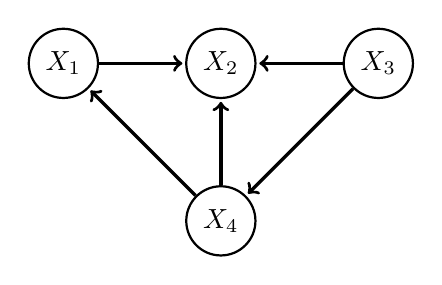
\begin{tikzpicture}[
            shorten > = 1pt, % don't touch arrow head to node
            auto,
            node distance = 2cm, % distance between nodes
            semithick % line style
        ]

        \tikzstyle{every state}=[
            draw = black,
            thick,
            fill = white,
        ]

        \node[state] (X1) {$X_1$};
        \node[state] (X2) [right of=X1] {$X_2$};
        \node[state] (X3) [right of=X2] {$X_3$};
        \node[state] (X4) [below of=X2] {$X_4$};
        \begin{scope}[very thick]

        \path[->] (X1) edge (X2);
        \path[->] (X3) edge (X2);
        \path[->] (X4) edge (X1);
        \path[->] (X4) edge (X2);
        \path[->] (X3) edge (X4);
\end{scope}
    \end{tikzpicture}
\end{center}

    $G_3$

\begin{center}
    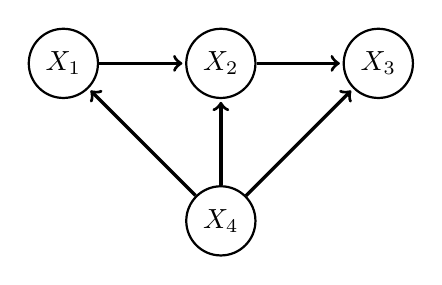
\begin{tikzpicture}[
            shorten > = 1pt, % don't touch arrow head to node
            auto,
            node distance = 2cm, % distance between nodes
            semithick % line style
        ]

        \tikzstyle{every state}=[
            draw = black,
            thick,
            fill = white,
        ]

        \node[state] (X1) {$X_1$};
        \node[state] (X2) [right of=X1] {$X_2$};
        \node[state] (X3) [right of=X2] {$X_3$};
        \node[state] (X4) [below of=X2] {$X_4$};
        \begin{scope}[very thick]

        \path[->] (X1) edge (X2);
        \path[->] (X2) edge (X3);
        \path[->] (X4) edge (X1);
        \path[->] (X4) edge (X2);
        \path[->] (X4) edge (X3);
\end{scope}
    \end{tikzpicture}
\end{center}


\maxmarks{5} \vspace{0 cm}

{\color{blue} $G_1$ and $G_2$ are equivalent. First of all, all three graphs
apparently have the same skeleton; $G_1$ has one unshielded collider $X_1$-$X_2$-$X_3$
V-configuration, so does $G_2$. However, $G_3$ doesn't have any such unshielded
collider V-configurations. Therefore $G_1$ and $G_2$ are equivalent. }



\clearpage

%%%%%%%%%%%%%%%%%%%%%%%%%%%%%%%%%%%%%%%%%%%
\question{3} {HMM I  (TA:- \myfirstta)}
You have already learned forward method and backward method to compute the probability for a given observed sequence: $P(O_1 ... O_T)$\\
In this problem, we want to give you a different perspective of view to do this job and will use this new way to compute some probabilities for the following example HMM.
\begin{figure}[h]
\centering
\begin{tabular}{cc}
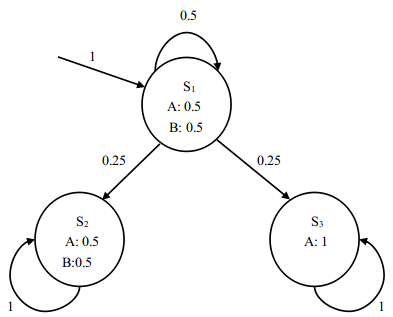
\includegraphics[width = 0.28\textwidth]{q3.jpg}& 
\end{tabular}\label{fig:GNB}
\end{figure}

\part{a}
Let $v_i^t=p(O_1 ... O_T|q_t=s_i)$. Write a formula for $P(O_1 ... O_T)$ using \textbf{only} $v_i^t$ and $p_t(i)$. [we define $p_t(i)$=$p(q_t=s_i)$]
\maxmarks{3}
{\color{blue} 
\begin{equation*}
	\Pr(O_1,\dots,O_T)=\sum_iP(O_1,\dots,O_T|q_t=s_i)p(q_t=s_i)
\end{equation*} }
\part{b}
Compute $p(O_1=B,...,O_2{}_0{}_0=B)$ (observing 200 B's in the sequence)
\maxmarks{6}\vspace{-6pt}

{\color{blue} {\bf Observation}: If the model is in $S_1$ at the $i$-th iteration, 
it can never reach any other states before that iteration - otherwise it won't be able
to go back to $S_1$; if the model ends up in state $S_2$, at some point $t=t_0$, 
the model will go from $S_1$ to $S_2$, with a probability of $0.25$. $q_{200}\ne S_3$
since the model in $S_3$ doesn't emit $B$. Also, as long as the model is in state 
$S_1$ or $S_2$, B emits with $\Pr=0.5$.
\begin{flalign*}
	\Pr(O_1=B,\dots,O_{200}=B)=&\Pr(O_1=B,\dots,O_{200}=B|q_{200}=S_1)\Pr(q_{200}=S_1) \\
		&+\Pr(O_1=B,\dots,O_{200}=B|q_{200}=S_2)\Pr(q_{200}=S_2) \\
		=&\,\left(0.5^{200}\right)\left(1\times0.5^{199}\right)+
		\left(0.5^{200}\right)\left(\textstyle\sum_{t_0=2}^{200}1\cdot0.5^{t_0-2}
		\cdot0.25\cdot1^{200-t_0}\right) \\
		=&\,0.5^{400}+0.5^{201}
\end{flalign*} }
\part{c}
Compute $p(O_1=A,...,O_2{}_0{}_0=A)$ (observing 200 A's in the sequence)
\maxmarks{6}\vspace{-6pt}

{\color{blue} {\bf Observation}: Use similar idea with (b), but note that here the model
can reach $S_3$ at some point, and the probabilities for emitting $A$ are different between 
$S_3$ and $S_1$. 
\begin{flalign*}
	\Pr(O_1=A,\dots,O_{200}=A)=&\Pr(O_1=A,\dots,O_{200}=A|q_{200}=S_1)\Pr(q_{200}=S_1) \\
		&+\Pr(O_1=A,\dots,O_{200}=A|q_{200}=S_2)\Pr(q_{200}=S_2) \\
		&+\textstyle\sum_{t_0=2}^{200}\left[
		\Pr(O_1=A,\dots,O_{200}=A|q_{200}=S_3,t=t_0)\Pr(q_{200}=S_3,t=t_0)\right] \\		
		=&\, \left(0.5^{200}\right)\left(1\times0.5^{199}\right)+
		\left(0.5^{200}\right)\left(\textstyle\sum_{t_0=2}^{200}1\cdot0.5^{t_0-2}
		\cdot0.25\cdot1^{200-t_0}\right) \\
		&+\left(\textstyle\sum_{t_0=2}^{200}0.5^{t_0-1}1^{200-(t_0-1)}
		\cdot1\cdot0.5^{t_0-2}\cdot0.25\cdot1^{200-t_0}\right) \\	
		=&\,\textstyle\frac16+\textstyle\frac13\cdot0.5^{400}+0.5^{201}
\end{flalign*} }

\clearpage

%%%%%%%%%%%%%%%%%%%%%%%%%%%%%%%%%%%%%%%%%%%
\question{4} {HMM II (TA:- \myfirstta)}
 Consider the HMM defined by the transition and emission probabilities in the table below. This HMM has six states (plus a start and end states) and an alphabet with four symbols (A,C,G and T). Thus, the probability of transitioning from state $S_1$ to state $S_2$ is 1, and the probability of emitting A while in state $S1$ is 0.5.\\
\begin{center}
    \begin{tabular}{| l | l | l | l | l | l | l | l | l || l | l | l | l |}
    \hline
    {} & 0 & $S_1$ & $S_2$ & $S_3$ & $S_4$ & $S_5$ & $S_6$ & $f$ & $A$ & $C$ & $G$ & $T$ \\ \hline
    0 & 0 & 1 & 0 & 0 & 0 & 0 & 0 & 0 & {} & {} & {} & {} \\ \hline
    $S_1$ & 0 & 0 & 1 & 0 & 0 & 0 & 0 & 0 & 0.5 & 0.3 & 0 & 0.2 \\ \hline
    $S_2$ & 0 & 0 & 0 & 0.3 & 0 & 0.7 & 0 & 0 & 0.1 & 0.1 & 0.2 & 0.6 \\ \hline
    $S_3$ & 0 & 0 & 0 & 0 & 1 & 0 & 0 & 0 & 0.2 & 0 & 0.1 & 0.7 \\ \hline
    $S_4$ & 0 & 0 & 0 & 0 & 0 & 0 & 0 & 1 & 0.1 & 0.3 & 0.4 & 0.2 \\ \hline
    $S_5$ & 0 & 0 & 0 & 0 & 0 & 0 & 1 & 0 & 0.1 & 0.3 & 0.3 & 0.3 \\ \hline
    $S_6$ & 0 & 0 & 0 & 0 & 0 & 0 & 0 & 1 & 0.2 & 0.3 & 0 & 0.5 \\
    \hline
    \end{tabular}
\end{center}
State whether the following are true or false and explain your answer.\\\\
\part{a}
$P(O_1=A, O_2=C, O_3=T, O_4=A, q_1=S_1, q_2=S_2)$ $=$\\$P(O_1=A, O_2=C, O_3=T, O_4=A|q_1=S_1, q_2=S_2)$
\maxmarks{4} \vspace{0 cm}

{\color{blue} TRUE. Since $p(q_1=S_1,q_2=S_2)=1$. }

\part{b}
$P(O_1=A, O_2=C, O_3=T, O_4=A, q_3=S_3, q_4=S_4)$ $>$ \\$P(O_1=A, O_2=C, O_3=T, O_4=A|q_3=S_3, q_4=S_4)$
\maxmarks{4} \vspace{0 cm}		

{\color{blue} FALSE. Since $p(q_3=S_3,q_4=S_4)=p(q_4=S_4|q_3=S_3)p(q_3=S_3)=p(q_3=S_3)<1$. }

\part{c}
$P(O_1=A, O_2=C, O_3=T, O_4=A, q_3=S_3, q_4=S_4)$ $<$ \\$P(O_1=A, O_2=C, O_3=T, O_4=A|q_3=S_5, q_4=S_6)$
\maxmarks{4} \vspace{0 cm}

{\color{blue} TRUE. Since LHS${}=1\cdot1\cdot0.3\cdot1\cdot0.7\cdot0.1<
1\cdot1\cdot0.3\cdot0.2={}$RHS}. 

\part{d}
$P(O_1=A, O_2=C, O_3=T, O_4=A)$ $>$ $P(O_1=A, O_2=C, O_3=T, O_4=A, q_3=S_3, q_4=S_4)$
\maxmarks{4} \vspace{0 cm}

{\color{blue} TRUE. Since LHS${}=\Pr(\dots,q_3=S_3,q_4=S_4)+\Pr(\dots,q_3=S_5,q_4=S_6)>{}$RHS. }

\part{e}
$P(O_1=A, O_2=C, O_3=T, O_4=A)$ $>$ $P(O_1=A, O_2=C, O_3=T, O_4=A|q_3=S_3, q_4=S_4)$
\maxmarks{4} \vspace{0 cm}

{\color{blue} FALSE. Since $\Pr(\dots,q_3=S_3,q_4=S_4)=0.7\cdot0.1
>0.3\cdot0.2=\Pr(\dots,q_3=S_5,q_4=S_6)$, so conditioning on $q_3=S_3,q_4=S_4$
actually results in a probability higher than average (LHS). }

\clearpage
%%%%%%%%%%%%%%%%%%%%%%%%%%%%%%%%%%%%%%%%%%%

\question{5} {HMM II (TA:- \myfirstta)}
 Consider the following two state HMM, answer the following questions. You can either get the answer by hand calculation or write a program to get the final answer.\\

\begin{figure}[h]
\centering
\begin{tabular}{cc}
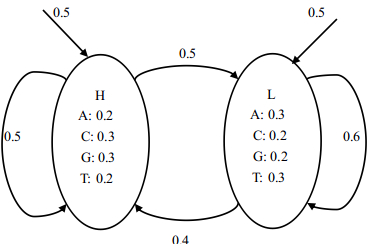
\includegraphics[width = 0.28\textwidth]{q5.jpg}& 
\end{tabular}
\caption{Figure of Q5}\label{fig:GNB}
\end{figure}

\part{a}
What is the probability for you to get an output sequence like \textbf{GGCA}
\maxmarks{7}

{\color{blue} 
$\Pr=0.0013767+0.0024665=0.0038432$. See {\tt po.m} for the code that gave this result.
}


\part{b}
What is the most likely hidden status sequence for the output sequence \textbf{GGCACTGAA}
\maxmarks{8}

{\color{blue}
See the table below for $\log_2\delta_t(j)$. Probabilities on the most probable path are italicized. \\
The most likely hidden status sequence is therefore {\tt HHHLLLLLL}. See {\tt pqao.m} for the code. 
\begin{table}[h!]
	\centering
	\begin{tabular}{cccccccccc} \toprule
	& G & G & C & A & C & T & G & A & A \\ \midrule
   H &\emph{-2.7370} & \emph{-5.4739} & \emph{-8.2109} &-11.5328 
   &-14.0068 &-17.3287 &-19.5396 &-22.8615 &-25.6574\\
   L &-3.3219 &-6.0589 &-8.7959 &\emph{-10.9479} &\emph{-14.0068} & \emph{-16.4807} & 
   \emph{-19.5396} & \emph{-22.0135} & \emph{-24.4874}
   	\\ \bottomrule
	\end{tabular}
\end{table}
}

\lstset{ %
  xleftmargin=12pt,
  xrightmargin=12pt,
  basicstyle=\scriptsize\tt, 
  commentstyle=\color{green!50!black},
  emphstyle=\color{red!50!black},
  stringstyle=\color{red!65!yellow!70!black},
  frame=single,
  keywordstyle=\color{blue}\bfseries,
  language=Matlab,
  numbers=left,
  numbersep=10pt,
  numberstyle=\color{black},
  title=\lstname
}

\lstinputlisting{po.m}
\lstinputlisting{pqao.m}

\clearpage		
%%%%%%%%%%%%%%%%%%%%%%%%%%%%%%%%%%%%%%%%%%%
\end{document}